% \chapter{How Holistic Co-Design Will Enable the Societal Uptake of Soft Robots}
\chapter{Safe yet Effective Soft Robots via Holistic Co-Design}
\label{chp:apx:holisticcodesign}

\begin{foreword}
    % In this thesis, we followed (so far) a traditional sequential design process: the soft robot's morphology, including structural shape, actuation, and sensor placement, was usually given and we assumed it to be fixed. Subsequently, we derived or learned reduced-order kinematic models and control-oriented dynamic models.
    % Finally, we leveraged the model knowledge within controllers and tuned their parameters (e.g., gains).
    % A good example for this sequential process are the \gls{HSA} which we extensively covered in this thesis: their design, including actuation, was done at the Distributed Robotics Lab (DRL) at MIT~\citep{lipton2018handedness, chin2018compliant, truby2021recipe}. Subsequently, as presented in Chapter~\ref{chp:hsamodel}, we derived kinematic and dynamical models from first principles, where we, particularly for the kinematic model, made extensive use of our intuition and prior experience, and subsequently determined their parameters via system identification.  Next, we devised model-based controllers in Chapter~\ref{chp:hsacontrol} and experimentally tuned their gains, and, finally, in Chapter~\ref{chp:braincontrol} developed a \gls{BMI} interface for guiding the low-level controller via brain signals measured with \gls{EEG} devices.
    % However, this sequential design process prevents from learnings and findings at later stages (e.g., during closed-loop control experiments) to influence the morphological design. This is a common issue in the larger soft robot community, where, for example, many designs are developed which are challenging to model via reduced order approaches and control precisely.
    % Instead, we consider in this appendix the co-design of the body (e.g., morphology) and the brain (e.g., control and perception algorithms) of soft robots which includes structured feedback mechanisms for iteratively optimizing the entire design of the soft robot. Specifically, we review the aspects currently lacking in soft robot co-design techniques and give suggestions how to resolve them via a proposed holistic co-design framework.
    In this thesis, we employed (so far) a traditional sequential design process: the soft robot’s morphology—including its structural shape, actuation, and sensor placement—was predefined and assumed fixed. We then derived or learned reduced-order kinematic and control-oriented dynamic models, leveraging this model knowledge within controllers whose parameters (e.g., gains) were subsequently tuned. A notable example of this process is the design of \gls{HSA} robots, extensively covered in this work. First, their design and actuation were developed at the Distributed Robotics Laboratory (DRL) at MIT~\citep{lipton2018handedness, chin2018compliant, truby2021recipe}. Subsequently, we developed in this thesis modeling and control approaches for such \gls{HSA} robots. In Chapter~\ref{chp:hsamodel}, we derived kinematic and dynamic models from first principles—relying heavily on our intuition and prior experience for the kinematic model—and determined their parameters via system identification. We then devised model-based controllers in Chapter~\ref{chp:hsacontrol} and experimentally tuned their gains, culminating in the development of a \gls{BMI} interface in Chapter~\ref{chp:braincontrol} to guide the low-level controller using EEG-measured brain signals.
    %
    However, this sequential process prevents insights gained during later stages, such as closed-loop control experiments, from influencing the morphological design. This is a common challenge within the soft robotics community, where many designs prove difficult to model with reduced-order approaches and control accurately. In this appendix, we instead consider the co-design of the body (morphology) and the brain (control and perception algorithms) of soft robots, incorporating structured feedback mechanisms to iteratively optimize the entire design. Specifically, we review current gaps in soft robot co-design techniques and propose solutions through a holistic co-design framework, which also considers the co-optimization of control-oriented reduced-order models and (model-based) controllers.
\end{foreword}

\pagebreak

\begin{abstract}
    % Soft robots promise inherent safety and embodied intelligence, enabling seamless interactions with both people and delicate environments. Yet their development remains challenging, as it requires integrating materials, geometry, actuation, and control into a cohesive design strategy. Despite recent progress, the field still struggles to balance task-specific performance with broader system-level considerations, often resulting in fragmented design approaches. For instance, lacking a quantitative safety metric, many designs are rendered overly soft—compromising crucial performance aspects such as motion precision and payload capacity. In this chapter, we propose a holistic co-design framework that transcends conventional optimization by viewing soft robots as inherently interconnected systems. Specifically, we call for the creation of a quantitative safety metric for soft robots, introduce techniques to significantly enhance computational efficiency in co-design, and advocate for moving beyond solely simulation-based evaluations by incorporating purposeful real-world prototyping. We believe that this holistic framework has the potential to greatly enhance the performance and overall value of soft robots while maintaining essential safety, ultimately redefining human-robot interaction and fostering greater acceptance and confidence in soft robotic systems.  
    % The development of soft robots remains particularly challenging, as it requires integrating materials, geometry, actuation, and autonomy stacks into a complex mechatronic system. Despite recent progress, the field still struggles to balance task-specific performance with broader system-level considerations, such as durability and manufacturability, often resulting in not sufficiently effective designs, that is at least partially a consequence of a traditional sequential design process.
    % Recently, co-design approaches that co-optimize the body and brain of soft robots have been started to be investigated.
    % However, while designing morphology and control together has lead to the identification of interesting unconventional designs, the existing methods have three major shortcomings: First, most approaches evaluate one task performance metric sin simulation, while a design that is effective and optimal in the real world needs to fulfill many more values.
    % Secondly, existing approaches focus on computational modeling of the design and ignore that the goal at the end is to realize the design into a mechatronic system whose actual performance might be degraded as a result of the sim-to-real gap.
    % Thirdly, existing approaches are computationally inefficient, therefore, not allowing an effective exploration of the full design space.
    % In this chapter, we propose a holistic co-design framework for soft robots that aims to resolve all three challenges by i) considering a broad of design values, ii) explicitly account for the realization of the design and how prototyping in the real world can help decrease the uncertainty in metrics that we use to optimize the design, iii) multiple modifications that have the potential to dramatically increase the computational efficiency, such as auxiliary metrics that are less expensive to evaluate or a model-based derivation of the control policy.
    % We believe that this holistic framework has the potential to greatly enhance the performance and overall value of soft robots, ultimately redefining human-robot interaction and fostering greater acceptance and confidence in soft robotic systems. 
    The development of soft robots remains particularly challenging, as it requires integrating materials, geometry, actuation, and autonomy stacks into a complex mechatronic system. Despite recent progress, the field still struggles to balance task-specific performance with broader system-level considerations—such as durability and manufacturability—often resulting in suboptimal designs, partly due to following a traditional sequential design process. Recently, co-design approaches that simultaneously optimize the body and brain of soft robots have begun to emerge. While combining morphology and control has revealed intriguing, unconventional designs, existing methods face three major shortcomings. First, most approaches rely on simulation-based evaluations that focus on a single performance metric, even though an effective real-world design must satisfy a broader range of values. Second, current methods concentrate on computational modeling without fully addressing the need to realize the design as a mechatronic system whose performance can be compromised by the sim-to-real gap. Third, these approaches are computationally inefficient, limiting the exploration of the full design space.
    In this chapter, we propose a holistic co-design framework for soft robots that tackles these challenges by (i) considering a wider array of design values, (ii) explicitly accounting for the realization of the design and how real-world prototyping can reduce uncertainties in evaluation metrics, and (iii) incorporating modifications that dramatically increase computational efficiency—such as using less expensive auxiliary metrics or adopting model-based control derivation. We believe this holistic framework has the potential to significantly enhance the performance and overall value of soft robots, ultimately redefining human-robot interaction and fostering greater acceptance and confidence in these systems.
\end{abstract}

\blfootnote{
    This chapter is partly based on \faFileTextO~\emph{\textbf{M. Stölzle}*, N. Pagliarani*, F. Stella*, J. Hughes, C. Laschi, D. Rus, M. Cianchetti, C. Della Santina, and G. Zardini (2025). Safe yet Effective Soft Robots via Holistic Co-Design. In Nature Machine Intelligence, \textbf{\emph{In Preparation}}}.

    % \nth{1}-author contributions: M. Stölzle conceived and led the project and wrote the vast majority of the content presented in this chapter. The other co-first-authors contributed ideas and were responsible for the graphics.

    $^*$M.S., N.P., and F.S. equally contributed to this work.
    M.S. conceived and led the project.
    All authors contributed ideas to this perspective.
    N.P., F.S., and M.S. collaborated on the figures and graphics.
    M.S. wrote the majority and N.P. and F.S. parts of the manuscript.
    All authors revised the manuscript.
    G.Z., C.D.S, M.C., and J.H. supervised the project and provided funding.
}

%% Start the actual chapter on a new page.
\newpage

\section{Introduction}
\begin{figure*}[ht]
    \centering
    \includegraphics[width=\textwidth]{appendix-holistic-codesign/figures/holistic_codesign_overview_v1.pdf}
    \caption{Co-design process for soft robotics, integrating task requirements and objectives, intelligent materials, embedded actuation, autonomy stack (e.g., control and perception systems), environmental considerations, and human-robot interaction to optimize both performance and safety for human-centric robotic applications.}
    \label{fig:apx:holisticcodesign:overview}
\end{figure*}

Soft robotic development is inherently complex, requiring the seamless integration of materials, geometry, actuation, and sensing with compliant continuum dynamics, perception, and control systems. Co-design strategies have proven effective in addressing multi-objective problems and accommodating the compositional, hierarchical nature of complex systems~\citep{zardini2023co}, thereby potentially allowing for finding the delicate balance between safety and performance. Successful co-design has been demonstrated in fields such as chemistry~\citep{norskov2009towards,vaissier2018computational}, construction engineering~\citep{knippers2021integrative}, articulated robotics~\citep{ha2018computational,zhao2020robogrammar}, and self-driving vehicles~\citep{zardini2021co}.
% 
Recent research has begun to develop co-design algorithms for soft robots that simultaneously optimize the body (e.g., morphology) and the brain (e.g., control and perception systems)~\citep{van2018spatial, spielberg2019learning, chen2020design, bhatia2021evolution, spielberg2021co, wang2023preco, medvet2021biodiversity, wang2022curriculum, junge2022leveraging, legrand2023reconfigurable, wang2024diffusebot, navez2024contributions}. However, several shortcomings limit their broader application. First, the optimization cycles are computationally expensive, hindering full design space exploration and global optimum identification, thus reducing practical utility~\citep{chen2020design}. This inefficiency arises from high-dimensional design spaces (e.g., voxel- or particle-based discretizations)~\citep{spielberg2019learning, medvet2021biodiversity, medvet2022impact, wang2022curriculum, legrand2023reconfigurable, wang2023softzoo, wang2023preco, wang2024diffusebot}, inefficient optimization routines (e.g., evolutionary algorithms)~\citep{chen2020design, rieffel2014growing, hiller2012automatic, bhatia2021evolution, medvet2021biodiversity, medvet2022impact}, and expensive control derivation via inner loops where a \gls{RL} controller is trained from scratch for each iteration~\citep{bhatia2021evolution, wang2022curriculum, wang2023softzoo, wang2023preco}, compounded by the reliance on computationally intensive simulations for evaluating the fitness of a design~\citep{spielberg2019learning, medvet2021biodiversity, medvet2022impact, wang2022curriculum, legrand2023reconfigurable, wang2023softzoo, wang2023preco, wang2024diffusebot}.
% 
Second, a narrow focus on easily computable evaluation metrics (e.g., locomotion speed, workspace) often neglects other vital design values such as usability, safety, cost, ecological impact, and regulatory requirements~\citep{junge2022leveraging}. For example, manufacturability is frequently overlooked, leading to voxel-based designs that are rarely practical to fabricate~\citep{legrand2023reconfigurable, wang2024diffusebot}.
% 
Third, evaluation metric uncertainty is seldom addressed~\citep{chen2020design}, resulting in designs that perform well in simulation but underperform in real-world scenarios.
% 
Finally, current co-design methods generally fail to incorporate diverse stakeholder input or account for end-user requirements.

The holistic co-design framework proposed in this chapter adopts a comprehensive view of design values and components, offering a path to address previous shortcomings of soft robotic co-design through several key modifications. First, it considers a wide range of requirements, objectives, and constraints—including safety, fabrication and operation costs, environmental impact, and regulatory restrictions. Second, we introduce enhancements to computational co-design that can significantly boost efficiency by (i) embracing reduced-order design spaces from which designs are sampled and decoded into full spatial morphologies~\citep{wang2024diffusebot}; (ii) co-optimizing reduced-order dynamical models—whether physics-based~\citep{armanini2023soft, alkayas2025soft} or learned~\citep{liu2024physics, stolzle2024input}—to capture the specific deformations experienced during tasks while minimizing model complexity; (iii) employing less expensive auxiliary metrics (e.g., controllability or observability based on the reduced-order model) that provide early feedback to eliminate likely underperforming designs; and (iv) replacing RL controllers trained from scratch with existing, more efficient model-based control techniques that exploit the reduced-order model~\citep{della2023model, stolzle2024input}. Third, we take a probabilistic view on co-design, acknowledging that evaluation metrics can be uncertain—due, for example, to the sim-to-real gap~\citep{dubied2022sim}—but that high-fidelity simulations and prototyping at varying \glspl{TRL}~\citep{NASA_TRL} can reduce this uncertainty. We formalize the tradeoff between "refinement" (computational optimization based on current metric beliefs) and "realization" (prototyping a design and acquiring true measurements for the evaluation metrics), paving the way for a resource-efficient holistic co-design strategy. Finally, early stakeholder involvement through structured consultations and iterative feedback ensures that practical insights on usability, manufacturability, and scalability are integrated, aligning design decisions with real-world criteria.

Illustrated in Fig.~\ref{fig:apx:holisticcodesign:overview}, this holistic co-design framework for soft robots has the potential to reshape societal norms by empowering robots to take on critical roles in caregiving, education, and other sensitive fields. By deploying more effective and high-performing soft robots in human-centric environments while ensuring the necessary safety, we can enhance human well-being, address key societal challenges, and foster broader societal acceptance of robots.
\section{The Past and Present Soft Robot Design Process}\label{sec:apx:holisticcodesign:related_work}

In this section, we review established design processes in the field of soft robotics. The discussion is organized into two parts: first, we examine the fundamental design cycle typically employed in soft robotics, covering the progression from initial task specifications to experimental prototyping and final design approval. Second, we explore recent work on the co-design of soft robots that showcases some initial ideas on how we could jointly design the body and brain.
% highlighting approaches aimed at integrating various design aspects more effectively in the development of soft robotic systems.

\subsubsection{Traditional Design Process of Soft Robots}
The basic design cycle typically described in the literature involves several key steps~\citep{roozenburg1995product, van2020delft}: (1) The cycle begins with defining criteria, where designers explicitly specify the values, requirements, and functions that the design must satisfy; (2) Next is the provisional design stage, in which solution ideas, concepts, and implementations are synthesized; (3) Following this, simulations can be used to anticipate the potential properties and performance of the design. These predictions are validated in step (4) by manufacturing prototypes at various \glspl{TRL}~\citep{NASA_TRL}; (5) Finally, if the prototypes meet the established criteria, the design is approved.

This traditional design process is also widely applied within soft robotics. As illustrated in Fig.~\ref{fig:apx:holisticcodesign:current_design_vs_holistic_codesign}~(Left), it begins with task specifications and proceeds to a preliminary conceptual design, followed by detailed mechatronic development. The open-loop behavior of the resulting design is verified through simulation, fabrication, and testing on breadboard prototypes. Typically, control design and reduced-order modeling occur only after validating a viable soft robotic prototype, enabling verification of closed-loop behavior within laboratory settings. Furthermore, steps (2)-(4) often involve iterative cycles of diverging and converging phases~\citep{feldhusen2013pahl}. During the \emph{diverging} phase, new design ideas, concepts, and implementations are generated. Conversely, the \emph{converging} phase evaluates these concepts through simulations or prototype tests to identify, for example, via selection matrices~\citep{ulrich2016product}, promising designs worthy of further development.

However, the traditional design cycle has several notable deficiencies:
(i) Although multiple iterations can theoretically "close the loop" of the design cycle, practical constraints—such as costs and complexity—often render iterative processes prohibitively expensive. Additionally, no formal or automated method typically exists to systematically incorporate insights from evaluated performance metrics back into improving the original design.
(ii) Similarly, divergence and convergence cycles frequently lack effective feedback mechanisms, preventing valuable knowledge acquired during detailed design or high-fidelity prototyping from informing the generation of new design solutions.
Indeed, for example, Suh's first axiom on design theory for systems argues that cycles should be avoided and functional requirements should be orthogonal to each other~\citep{suh1998axiomatic}.
% However, many examples in practice in product development have demonstrated how an iterative approach can significantly improve products over time.
However, numerous practical examples in product development have shown that iterative approaches can substantially enhance product quality and performance and decrease cost over time. Therefore, a design process for soft robots should embed such feedback mechanisms from the beginning.
(iii) Constraints and metrics critical in later stages, such as manufacturability and compliance with regulatory standards, such as \gls{ISO} norms, are often inadequately considered during initial stages.
(iv) The sequential workflow between mechatronic design, perception, modeling, and control teams creates informational silos. For instance, modeling engineers typically transfer completed models to control engineers without sufficient feedback channels, thus restricting iterative enhancements.
(v) A significant drawback of conventional design processes is the potential loss of "design history." Critical insights, rationale for decisions, and trade-offs are frequently undocumented, particularly when team members transition roles or leave the project. Consequently, revisiting earlier stages or building on previous knowledge becomes increasingly challenging. For example, a research team seeking to modify an earlier actuator design after identifying field performance issues may find the original design rationale inaccessible.

\subsubsection{Co-Design of Soft Robots}
Given the complexity of soft robots and the limitations of traditional design processes—especially the absence of structured and effective feedback cycles and the isolated design of components—the community has recently begun exploring how co-design algorithms could support soft robot development~\citep{spielberg2019learning, cianchetti2021embodied, bhatia2021evolution, van2022co, wang2022curriculum, wang2023preco, wang2024diffusebot, junge2022leveraging}.
% The term "\textit{co}-design" can emphasize several difference compared to traditional design approaches, including a \textit{co}mpositional and hierarchical nature (i.e., designing all components of a system together), a \textit{co}llaborative approach involving all teams and stakeholders, an a \textit{co}ntinuous improvement of the design~\citep{zardini2023co}.
The term “\textit{co}-design” highlights several distinctions from traditional design approaches, including a \textit{co}mpositional and hierarchical nature - i.e., designing all system components, such as body and brain, together~\citep{junge2022leveraging}; a \textit{co}llaborative approach involving all teams and stakeholders, and a \textit{co}ntinuous process of design improvement~\citep{zardini2023co}.
Co-design strategies have proven highly effective at solving complex, possibly multi-objective, optimization problems with a well-defined design space, cost function, and equality/inequality constraints. 
Notable examples stem from the fields of chemistry~\citep{norskov2009towards,vaissier2018computational}, construction engineering~\citep{knippers2021integrative}, mobility systems~\citep{zardini2020co, zardini2022co}, autonomous vehicles~\citep{zardini2023co,zardini2021co}, articulated robotics~\citep{ha2018computational,zhao2020robogrammar}.
% Progress has been made in developing co-design algorithms for soft robots~\citep{van2018spatial, legrand2023reconfigurable, wang2024diffusebot}, but current approaches lack computational efficiency (specifically in modeling and control), offer limited optimality guarantees, and often cover only selected components of the design (e.g., exclude sensing, actuation or control).
% Furthermore, the generated designs can rarely be fabricated.\\

Initial attempts have applied co-design methods to soft robots by simultaneously optimizing the body/morphology (i.e., structural shape, actuation, and sensing) and the brain (e.g., controller)~\citep{spielberg2019learning, cianchetti2021embodied, bhatia2021evolution, van2022co, wang2022curriculum, wang2023preco, navez2024contributions, wang2024diffusebot, junge2022leveraging}. Drawing on extensive research in mechanical and morphological design—particularly geometric design—these approaches can be classified~\citep{chen2020design} into three categories: (a) size optimization, which focuses on regular shapes defined by (hand-picked) geometric parameters (e.g., radii, segment lengths, pneumatic chamber dimensions)~\citep{dammer2018design, wang2018programmable, guan2023trimmed, calisti2011octopus, pagliarani2024variable, polygerinos2015modeling, navez2024design, junge2022leveraging}; (b) shape optimization, which incrementally modifies the parametric surfaces of an initial design while preserving its connectivity or topology~\citep{siefert2019bio}; and (c) full topology optimization, which rethinks the structure entirely by creating, repurposing, or removing elements from the topology~\citep{sigmund2013topology, jewett2019topology, zhang2018topology, caasenbrood2020computational, spielberg2019learning, wang2022curriculum, legrand2023reconfigurable, wang2023softzoo, wang2023preco, wang2024diffusebot, pinskier2024diversity}.

However, the existing co-design approaches exhibit several shortcomings:
(i) The current topology optimization approaches often oversimplify the design process by discretizing the morphology spatially into passive, actuated, or sensorized voxels or particles~\citep{spielberg2019learning, medvet2021biodiversity, medvet2022impact, wang2022curriculum, legrand2023reconfigurable, wang2023softzoo, wang2023preco, wang2024diffusebot}, resulting in designs that rarely translate effectively to practical applications~\citep{legrand2023reconfigurable, wang2024diffusebot}. Additionally, (ii) most existing methods train learning-based controllers (e.g., using \gls{RL}) from scratch for each iteration, creating a significant computational bottleneck in the overall co-design cycle~\citep{bhatia2021evolution, wang2022curriculum, wang2023preco}. Recent progress in differentiable physics-based simulation~\citep{coevoet2017software, hu2019chainqueen, fang2020kinematics} suggests that integrating real-time gradient-based optimization of neural-network parametrized controllers could significantly reduce the computational overhead associated with iterative design-control loops, improving sample efficiency and convergence speed~\citep{spielberg2019learning, bacher2021design, wang2024diffusebot}. However, these methods assume smooth, end-to-end differentiability—which can fail under contact or discontinuities—and can be prone to local minima. 
Relatedly, (iii) these approaches typically require completing an entire cycle—from design generation, control policy training, and high-fidelity simulation through task-specific performance evaluation—before updating the design. This sequence can be highly computationally demanding and results in unnecessary resource use for designs that could have been earlier identified as suboptimal through intermediate metrics. 
% While “learning-in-the-loop” co-design~\citep{spielberg2019learning} reduces redundant evaluations by jointly optimizing morphology and control, a key drawback is its heavy reliance on simulation accuracy. 
Finally, (iv) most studies predominantly focus on computationally implementable aspects of the design process (i.e., \emph{computational co-design}), neglecting critical downstream considerations~\citep{junge2022leveraging} such as breadboard testing, validation with prototypes, or regulatory compliance. Although topology optimization and multi-material design techniques~\citep{chen2020design} are gaining traction, their integration with fabrication constraints remains an open challenge. Considering manufacturability from the early stages of co-design—particularly in the context of additive manufacturing- could enhance the feasibility of computationally optimized soft robots~\citep{navez2024contributions}.
However, we conclude that the high computational demands of co-design caused by computationally expensive simulations and inefficient optimization routines currently restrict its practical usefulness, limiting the scope of the design space that can be explored within available computing budgets~\citep{chen2020design}.
\section{A Framework for Holistic Co-Design}\label{sec:apx:holisticcodesign:holistic_co_design_framework}
\begin{figure}[h!]
    \centering
    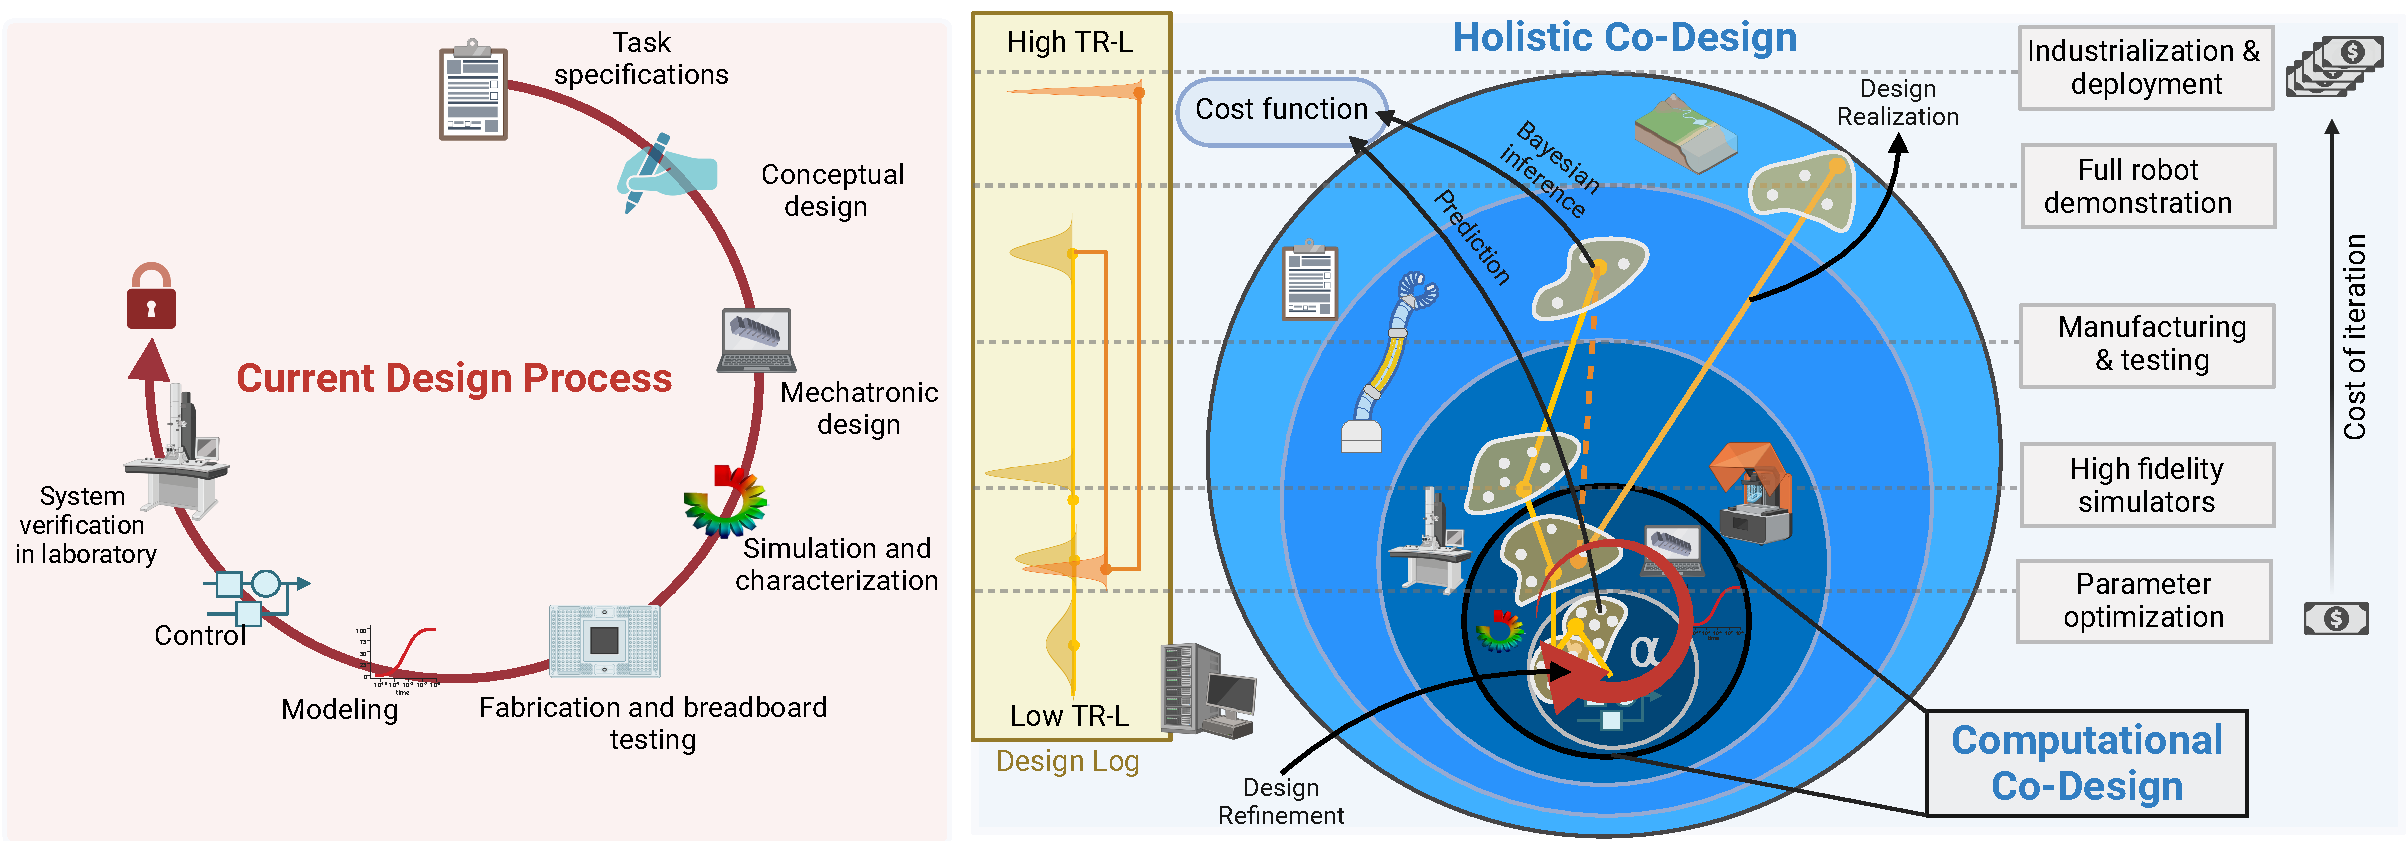
\includegraphics[width=1\linewidth]{appendix-holistic-codesign/figures/current_design_vs_holistic_codesign_v1.pdf}
    \caption{
        \textbf{Left:} A basic design cycle applied to soft robots, which mirrors how soft robots have been traditionally developed. It follows a very sequential approach and lacks feedback loops to iteratively and efficiently improve the design.
        \textbf{Right:} The holistic design contains different layers where the design is co-optimized, considering the cost of a new analysis and the relative reduction in uncertainty associated.
    }
    \label{fig:apx:holisticcodesign:current_design_vs_holistic_codesign}
\end{figure}

Holistic co-design marks a significant shift in soft robotics by adopting an integrated, application-driven strategy that emphasizes the seamless interaction between a robot’s physical morphology, its control system, and user engagement. Unlike traditional design cycles—which remain prevalent—it provides a structured framework that concurrently develops all system components, refining the design iteratively through effective feedback loops. Moreover, this approach distinguishes itself from other co-design methods by embracing a broader set of design values, advocating for cross-disciplinary collaboration and active participation from diverse stakeholders, introducing techniques to enhance computational efficiency, and proposing a probabilistic view that acknowledges uncertainties in evaluation metrics while outlining strategies to mitigate them as the design evolves.

In detail, the proposed holistic co-design framework introduces several key innovations. First, it optimizes a range of design attributes simultaneously—such as task completion time, safety, material and fabrication costs, energy consumption, and environmental impact—instead of focusing on a single metric like locomotion speed, as most current approaches do. Second, it significantly boosts the efficiency of computational co-design by (i) establishing a reduced-order design space that avoids the complexity of directly optimizing a high-dimensional spatial morphology (as seen in voxel-based methods); (ii) developing a control-oriented reduced-order model within the co-design process; (iii) employing computationally inexpensive auxiliary metrics, such as controllability, observability (leveraging the reduced-order model), or manufacturability, which provide early feedback to the optimizer instead of relying solely on the outcome of resource-intensive closed-loop simulations; and (iv) efficient derivation/learning of controllers based on the reduced-order model (i.e., model-based control).
Furthermore, while existing methods typically address only the fully computational aspects of design and evaluation, our framework explicitly accounts for the inherent uncertainties in these metrics—uncertainties that can only be properly identified through high-fidelity simulations or, ideally, extensive testing with physical prototypes. By introducing a probabilistic evaluation of a design’s “fitness,” we also formalize strategies to reduce such uncertainties through prototyping, as visualized in Fig.~\ref{fig:apx:holisticcodesign:current_design_vs_holistic_codesign}~(Right). Additionally, we emphasize that collaboration among team members with varied expertise and backgrounds, as well as engagement with stakeholders (including customers, scientific advisors, and domain experts), is essential for developing a high-performing soft robot. Finally, we conclude that co-design approaches not only help preserve design knowledge but also enhance reproducibility, addressing a well-known challenge in soft robotics~\citep{baines2024need}.

\paragraph{Multi-Objective Co-Design: Satisfying Comprehensive Requirements and Evaluation Metrics}
Current co-design approaches for soft robots typically consider only one, or at most a few, evaluation metrics\footnote{Commonly, such evaluation metrics are also referred to as costs, losses, or rewards} per task~\citep{spielberg2019learning, spielberg2021co, medvet2022impact, wang2023preco, wang2024diffusebot, navez2024design}. For locomotion tasks, this often means measuring the velocity achieved or the distance traveled in a fixed time period~\citep{spielberg2019learning, wang2023preco}, while in manipulation tasks (e.g., pushing), the focus is on how far an object is safely moved~\citep{wang2024diffusebot}. However, as soft robots evolve from research prototypes into commercial products, a broader set of design values becomes critical. These include, but are not limited to, safety (as discussed in Chapter~\ref{chp:safetymetric}), manufacturing costs (especially in relation to production batch sizes)~\citep{miriyev2017soft, schmitt2018soft, majidi2014soft, junge2022leveraging}, material supply, and the robot’s operational lifetime—which depends on both the materials used and the stresses experienced—as well as ecological and recycling considerations~\citep{mazzolai2020vision}. Additionally, regulatory requirements grow in significance; traditional design processes tend to address regulatory standards only at the end or not at all, whereas regulatory compliance is essential from the start. For example, medical soft robots must meet the FDA or EMA guidelines, which dictate acceptable materials, manufacturing methods, and performance criteria. Incorporating these regulatory factors into the design optimization loop helps prevent late-stage redesigns that could delay product deployment and significantly increase development costs. Holistic co-design integrates these values and constraints from the beginning, ensuring that the resulting designs are optimal across all dimensions.

\paragraph{Increasing the Efficiency of Computational Co-Design}
\emph{Computational co-design} for soft robots refers to developing an automatic algorithm that optimizes the integrated design (encompassing both body and control components) to meet specified performance criteria and design values~\citep{carlone2019robot, wang2023softzoo}. In its most general form, co-design can be formulated as a constrained nonlinear optimization problem~\citep{zardini2023co} over a parameterized design $x$, such that
\begin{equation}
\begin{aligned}
    \min_{x} \quad & f(x)\\
    \textrm{s.t.} \quad & g(x) = 0 \\
    & h(x) \leq 0,
\end{aligned}
\end{equation}
where $f(x): \mathcal{X} \to \mathcal{C}$ represents the cost or loss function, and $g(x): \mathcal{X} \to \mathbb{R}^{n_\mathrm{eq}}$ and $h(x): \mathcal{X} \to \mathbb{R}^{n_\mathrm{ineq}}$ denote the equality and inequality constraints, respectively. For example, in multi-objective optimization, we can define $f(x) = \begin{bmatrix} \hat{c}_1^\top(x), \dots, \hat{c}_{n_\mathrm{obj}}^\top(x) \end{bmatrix}^\top$, with each $f_j(x) = \hat{c}_j(x)$ for $j = 1, \dots, n_\mathrm{obj}$ corresponding to design objectives implemented via the (estimated) evaluation metrics $\hat{c}_j(x): \mathcal{X} \to \mathcal{C}_j$. These objectives might include task performance, manufacturing, and operational costs, or environmental impact. Equality constraints typically capture system dynamics, while inequality constraints ensure physical feasibility (such as non-negative volume, adherence to manufacturing tolerances, or minimum geometric dimensions for manufacturability) and guarantee that the design satisfies essential requirements (like minimum safety levels or regulatory standards). Please note that such (inequality) constraints can also be a function of an estimated evaluation metric $\hat{c}_j(x)$.

In our view, one key reason co-design approaches are not yet widely adopted in soft robotics is their computational inefficiency and high cost, which severely restrict the design space that can be explored and diminish the chances of finding the optimal design, thereby reducing their practical utility~\citep{chen2020design}. We identify three primary sources of computational inefficiency in current methods: (i) they often operate in high-dimensional design spaces—for instance, by discretizing the soft robotic geometry into voxels—which makes it extremely challenging, if not impossible, to locate the global optimum; (ii) the optimization loop is closed via performance metrics obtained from one or multiple closed-loop system simulations, and using high-fidelity simulators makes this evaluation process computationally demanding; (iii) assessing closed-loop performance requires access to a controller. In principle, there are two ways to address this: one can train a controller over a set of different designs~\citep{zardini2021seeking, boekel2025learning}, though this means the controller may not be optimized for a specific design, so the evaluation might not reflect the true performance achievable with a specialized controller. Alternatively, training a controller tailored to the proposed design can fully exploit its kinematics and dynamics to achieve optimal task performance, but this approach is computationally very intensive—especially when using \gls{RL} controllers trained from scratch~\citep{bhatia2021evolution, wang2022curriculum, wang2023softzoo, wang2023preco} or control policies trained via gradient descent using a differentiable simulation~\citep{spielberg2019learning, wang2023softzoo, wang2024diffusebot}—which often struggle with complex hybrid dynamics such as contact.

Our framework, depicted in Fig.~\ref{fig:apx:holisticcodesign:computational_co_design}, paves the way for significantly more efficient computational co-design of soft robots by introducing four key modifications that address the previously mentioned challenges:
% 
(1) Building on previous work~\citep{spielberg2019learning, wang2024diffusebot}, we advocate for performing optimization in a reduced-order design space, which can be either entirely learned or partially defined manually (e.g., specifying the length and diameter of a soft segment). In practice, reduced-order designs $x$ are sampled from a distribution, and then a design decoder reconstructs the full design description (such as a volumetric mesh with sensor and actuator placement). After evaluating the design, the optimizer updates the posterior belief of the sampling distribution to bias it towards effective designs. We elaborate on reduced-order design in Section~\ref{sec:apx:holisticcodesign:reduced_order_design_parametrizations}.
% 
(2) A control-oriented reduced-order model can greatly assist in analyzing the system’s motion characteristics and behavior~\citep{bruder2020data, armanini2023soft, menager2023direct, alora2023data, stolzle2024input, alkayas2025soft, valadas2025learning}. While deriving such models for rigid manipulators is generally straightforward~\citep{siciliano2010robotics, zhao2020robogrammar}, soft robotics presents an inherent interplay between design, actuation, and task (e.g., payload, gravitational forces) on one side and the resulting deformations on the other. This interdependence makes it essential to jointly synthesize the design (including actuation) and the kinematic model. We discuss this further in Sec.~\ref{sec:apx:holisticcodesign:codesigning_physical_intelligence}.
% 
(3) To reduce the reliance on performance metrics derived from resource-intensive closed-loop simulations, we introduce several auxiliary metrics that are computationally cheaper to evaluate. These metrics provide early feedback to the optimizer, allowing for the early discarding of designs with very low predicted fitness. Examples include metrics assessing observability and controllability based on the reduced-order model (which directly links actuator and sensor placement to the structural design), open-loop compliance~\citep{guan2023trimmed}, safety (as discussed in Chapter.~\ref{chp:safetymetric}), embodied intelligence~\citep{cianchetti2021embodied, mengaldo2022concise, vihmar2023measure}, or heuristics estimating manufacturability. We further discuss controllability and observability metrics in Sec.~\ref{sec:apx:holisticcodesign:codesigning_physical_intelligence}.
%
(4) Finally, we propose leveraging the reduced-order model to derive the control law in a model-based fashion. Recent advancements provide a solid foundation for exploiting dynamical models—whether physics-based or data-driven—for control~\citep{della2023model, laschi2023learning}. For example, using Koopman theory to learn a linear model (or linearizing a nonlinear model around equilibrium) enables the design of optimal controllers in closed form via LQR~\citep{bruder2020data}. For nonlinear models with a physical structure (i.e., with well-defined kinetic and potential energy terms)~\citep{armanini2023soft, liu2024physics, stolzle2024input, alkayas2025soft, valadas2025learning}, PID+Feedforward~\citep{della2023model, stolzle2024experimental, stolzle2024input} or similar closed-form controllers (e.g., PD+~\citep{della2020model}, computed torque) can be designed. When dynamics are modeled as generic nonlinear transition functions (e.g., \glspl{RNN}~\citep{thuruthel2017learning}, \glspl{NODE}~\citep{kasaei2023data}), optimal control techniques such as \gls{MPC}~\citep{alora2023data} or model-based \gls{RL}~\citep{thuruthel2018model} can compute the control input. These model-based approaches to deriving a control law are dramatically more computationally efficient than training an \gls{RL} control policy from scratch for each design~\citep{bhatia2021evolution, wang2022curriculum, wang2023softzoo, wang2023preco}.

\begin{figure}[h!]
    \centering
    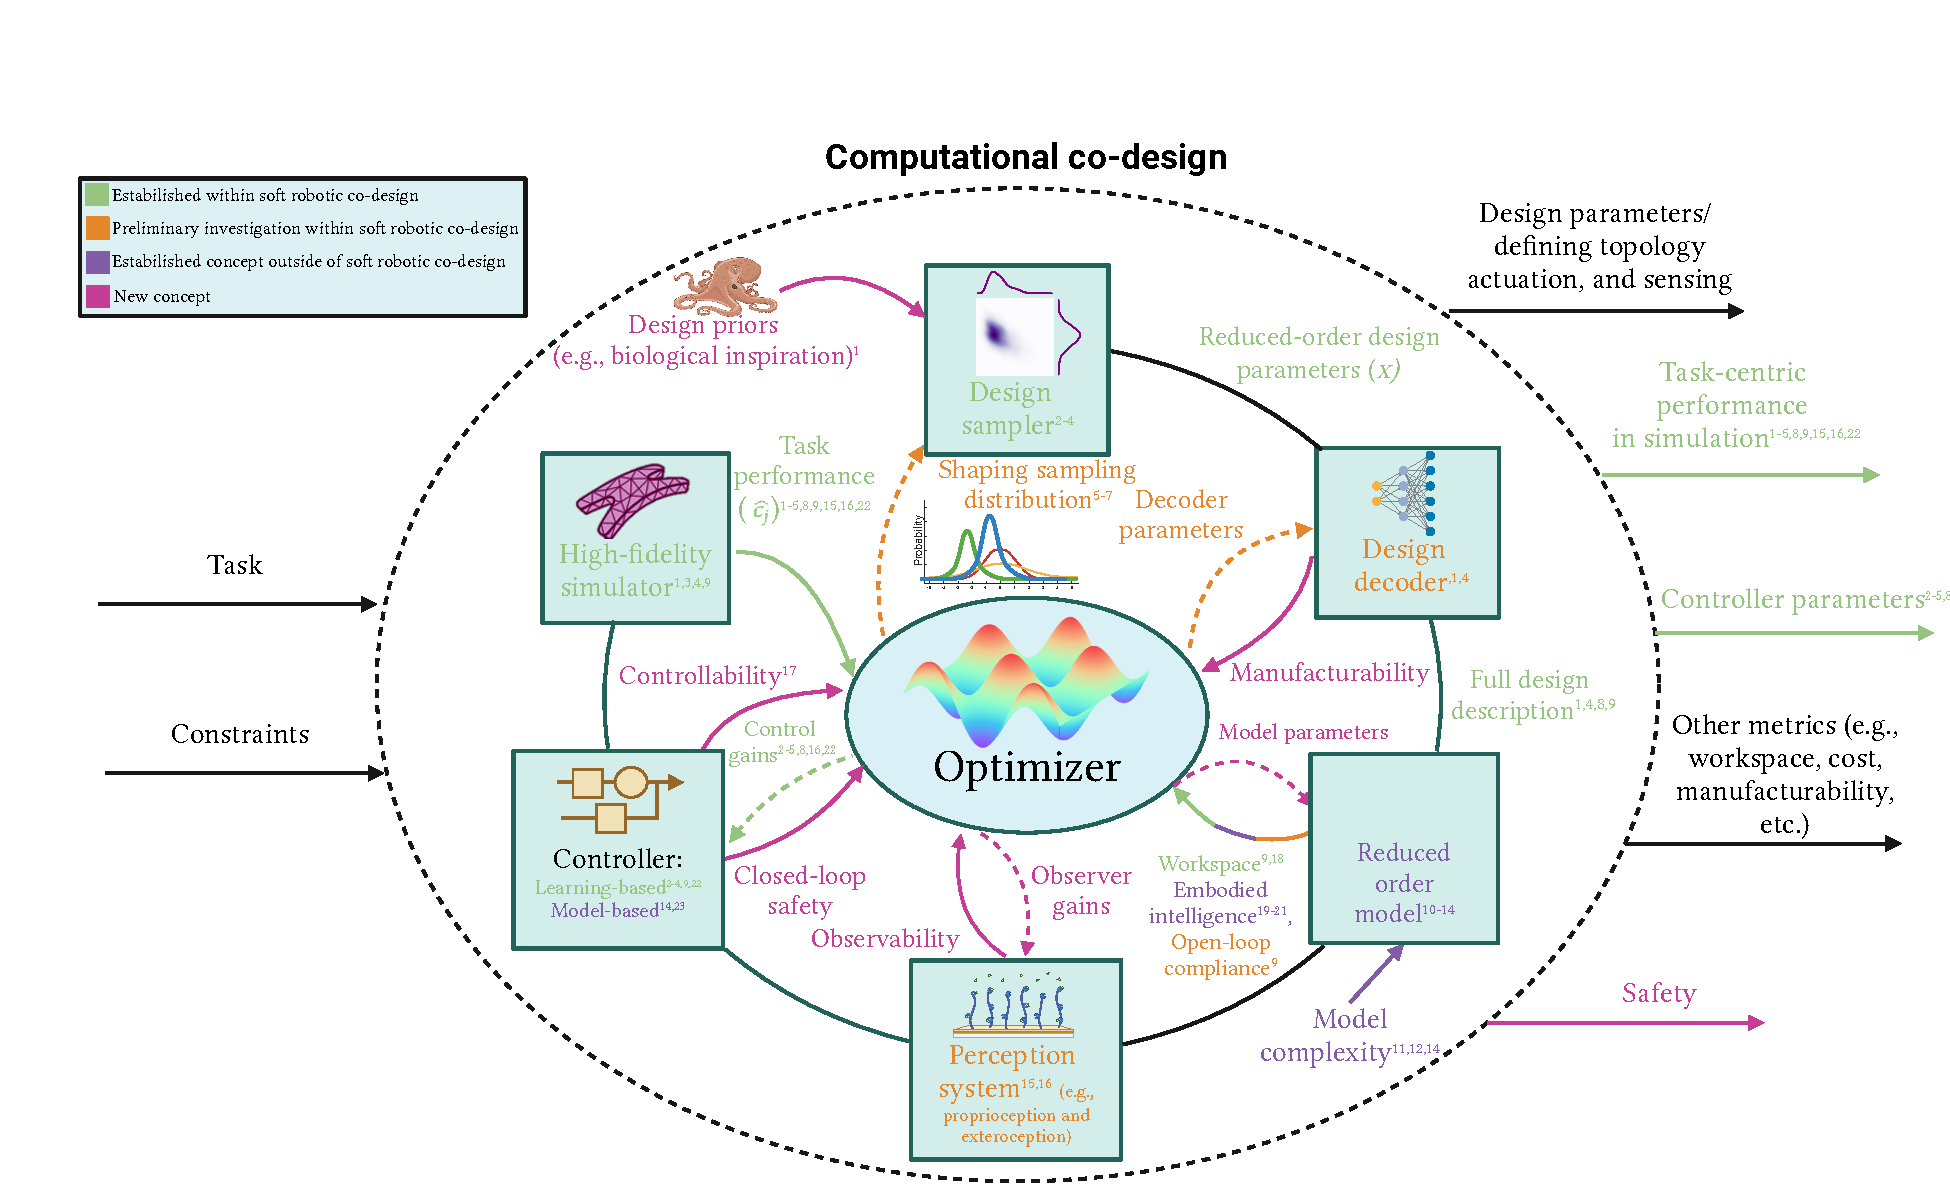
\includegraphics[width=1\linewidth]{appendix-holistic-codesign/figures/computational_codesign_v1.pdf}
    \caption{\textbf{A Framework for Efficient Computational Co-Design of Soft Robots:}
        We sample reduced-order design parameters $x$ from an initial distribution, which can incorporate design priors from biological inspiration~\citep{mazzolai2020vision, chen2020design, laschi2024bioinspiration} or existing effective soft robots. This reduced-order design space can either be fully learned or defined explicitly with physical or geometric meanings (e.g., number, radius, and length of segments). A design decoder then translates these parameters into a detailed description of the robot’s body, such as a volumetric mesh of the shape, including sensor and actuator placements. This description already provides rapid feedback on manufacturability and other design considerations. Subsequently, a reduced-order model (e.g., based on \gls{GVS}~\citep{renda2020geometric} dynamics) is derived or learned, enabling efficient preliminary evaluation of workspace, open-loop compliance, and embodied intelligence~\citep{cianchetti2021embodied, mengaldo2022concise, vihmar2023measure}, thus offering computationally inexpensive feedback to the optimizer. Similarly, perception and control systems can be derived or learned, with the reduced-order model facilitating efficient controller development (e.g., via model-based control~\citep{della2023model}, \gls{MPC}~\citep{alora2023data}, or gradient-based optimization via differentiable physics~\citep{spielberg2019learning, wang2023softzoo}). Additionally, the observability and controllability of the design can be assessed efficiently without costly simulations. Finally, closed-loop simulations, either low-fidelity (using the reduced-order model) or high-fidelity (\gls{FEM}-based~\citep{coevoet2017software}), assess the robot’s integrated task-centric performance (e.g., task completion time, energy consumption). These evaluations inform the optimization of the design sampling distribution, design decoder parameters, and all relevant parameters of the reduced-order model, perception, and control systems. \emph{References in graphic:}  
        (1):~\citep{navez2024contributions}, (2):~\citep{bhatia2021evolution}, (3):~\citep{wang2023softzoo}, (4):~\citep{wang2024diffusebot}, (5):~\citep{song2024morphvae}, (6):~\citep{sutton1998reinforcement}, (7):~\citep{garnett2023bayesian}, (8):~\citep{medvet2022impact}, (9):~\citep{guan2023trimmed}, (10):~\citep{armanini2023soft}, (11):~\citep{valadas2025learning}, (12):~\citep{alkayas2025soft}, (13):~\citep{menager2023direct}, (14):~\citep{alora2023data}, (15):~\citep{spielberg2021co}, (16):~\citep{junge2022leveraging}, (17):~\citep{zheng2019controllability}, (18):~\citep{amehri2022workspace}, (19):~\citep{cianchetti2021embodied}, (20):~\citep{mengaldo2022concise}, (21):~\citep{vihmar2023measure}, (22)~\citep{spielberg2019learning}, (23):~\citep{della2023model}.
        % (1) Navez, \emph{PhD Thesis}, 2024 (2) Bhatia et al., \emph{NeurIPS}, 2021 (3) Wang et al., \emph{ICLR}, 2023 (4) Wang et al., \emph{NeurIPS}, 2023 
        % (5) Song et al., \emph{AAAI}, 2024 (6) Sutton Barto, \emph{MIT Press}, 2015
        % (7) Garnett Roman, \emph{Cambridge University Press}, 2023 (8) Medvet et al., \emph{GECCO}, 2022 (9) Guan et al., \emph{npj Robotics}, 2023 (10) Armanini et al., \emph{T-RO}, 2023 (11) Valadas et al., \emph{RoboSoft}, 2025 (12) Alkayas et al., \emph{T-RO}, 2025
        % (13) Ménager et al., \emph{ICRA}, 2023 (14) Alora et al., \emph{ICRA}, 2023
        % (15) Spielberg et al., \emph{Co-Learning}, 2021 (16) Junge et al., \emph{EI}, 2022 (17) Zheng et al., \emph{ICRA}, 2019 (18) Amehri, \emph{PhD Thesis}, 2023
        % (19) Cianchetti, \emph{Front. Robot. AI}, 2021, (20) Mengaldo et al., \emph{Nature Reviews Physics}, 2022
        % (21) Vihmar et al., \emph{EI}, 2022 (22) Spielberg et al., \emph{NeurIPS}, 2019
        % (23) Della Santina et al., \emph{Contr. Syst. Mag.}, 2023.
    }
    \label{fig:apx:holisticcodesign:computational_co_design}
\end{figure}

\paragraph{Probabilistic Evaluation Metrics}
Another key tenet of holistic co-design is the explicit recognition of uncertainty when evaluating a design computationally across multiple dimensions~\citep{chen2020design}. In contrast to many existing approaches~\citep{wang2024diffusebot} that rely on one or a few metrics derived from simulations as stand-ins for a design’s actual performance, our perspective acknowledges that such performance metrics estimated via simulation are only proxies. For example, the DiffuseBot study~\citep{wang2024diffusebot} assesses various robotic tasks—such as balancing, landing, crawling, gripping, and box manipulation—using performance metrics based on closed-loop simulation outcomes. However, the well-known sim-to-real gap~\citep{dubied2022sim} means that a design’s simulation performance often deviates from its real-world behavior~\citep{junge2022leveraging}. Moreover, important factors like manufacturing costs~\citep{junge2022leveraging}, ecological sustainability, or the operational lifetime of a soft robot are difficult to evaluate solely through simulation and instead require prototyping, verification, and real-world testing, often with human involvement. As a result, the “optimal” design identified through computational co-design may not be optimal in practice.

To address these challenges, we propose a framework that adopts a probabilistic view of evaluation metrics—treating them as probabilistic beliefs about expected performance conditioned on the design specifications. This approach enables us to (a) explicitly account for uncertainty in the metrics during the design optimization process, (b) optimize the design also based on metrics that cannot be directly evaluated in simulation (e.g., manufacturability), and (c) progressively build confidence in the metrics and reduce uncertainty through high-fidelity simulations and/or prototyping. 
In our framework, the optimization process leverages the current probabilistic estimates of the metrics (i.e., refinement) to assess and improve designs computationally while using prototyping and experimental validation to refine these metric estimates (i.e., realization). This balance draws on well-established techniques from Bayesian optimization and reinforcement learning to manage the trade-off between refinement and realization effectively.
% In Fig.~\ref{fig:holistic_co_design}~(Right), refinement is visualized as design iteration cycles within the inner-most layer, and realization as, for selected designs, transitioning to the outer layers by building prototypes with varying TR-Ls and gaining confidence in the evaluation metrics and designs as a result.
In Fig.~\ref{fig:apx:holisticcodesign:current_design_vs_holistic_codesign}~(Right), refinement is depicted as the iterative design cycles within the innermost layer, while realization is shown by selected designs transitioning to the outer layers—achieved through building prototypes with varying TR-Ls to enhance confidence in both the evaluation metrics and the designs.
Ultimately, this methodology ensures that resources are allocated efficiently by prioritizing prototyping and testing in areas where predictive confidence is low but the potential for outstanding real-world performance is high. We discuss this approach in greater detail in Sec.~\ref{sec:apx:holisticcodesign:probabilistic_co_design_metrics}.


\paragraph{Synergistic Cross-Disciplinary Collaboration}
Collaboration is another pillar of this co-design process. The approach actively involves diverse stakeholders, engineers, end-users, material scientists, and domain experts from the outset. This collective input ensures that requirements are practical and adaptable to real-world constraints. For instance, when designing a robotic arm for harvesting, growers provide insights into crop fragility and harvesting techniques, guiding the development of soft end-effectors that minimize damage and maximize yield.

In traditional design workflows, this kind of collaboration is often sequential: the modeling engineer finishes their work and hands it over to the control engineer, who then applies control strategies without sufficient feedback loops. This hand-off model creates information silos and limits opportunities for iterative improvement. In contrast, co-design promotes continuous communication between these roles. For instance, the modeling engineer and the control engineer work in tandem, iterating on the design as new insights emerge, resulting in a more refined final product.

\paragraph{Preserving Design Knowledge and Enabling Reproducibility}
A significant drawback of conventional design processes is the potential loss of the "design history". Key insights, decisions, and trade-offs often remain undocumented, especially when team members leave or shift roles. As a result, revisiting earlier design stages or learning from past iterations becomes challenging or even impossible. For instance, if a research team wants to tweak a previously tested actuator geometry after realizing performance limitations in the field, they might discover that the rationale behind the original design choices is no longer accessible.

Holistic co-design naturally addresses this issue by serving as a transparent log of the development process. Design discussions, iterations, and parameter choices are recorded throughout the project, creating an accessible "audit trail". If a team needs to revisit an earlier design step, they can do so with clarity, regardless of team turnover or changing project priorities. Furthermore, the audibility significantly eases the certification process, which we already discussed previously.

In a co-design approach, however, the process remains inherently flexible. Since parameter definitions, performance assessments, and stakeholder inputs are continuously documented, engineers can backtrack when needed to refine or adjust the design by recalibrating safety margins based on updated risk analyses, testing alternative hardware configurations to optimize for cost or power consumption, or revisiting software algorithms in response to emerging performance data. This iterative workflow inherently aligns technical feasibility, regulatory compliance, and evolving business objectives in a transparent manner, ensuring that every modification is grounded in both empirical evidence and strategic considerations.
\section{Reduced-Order Design Parametrizations}\label{sec:apx:holisticcodesign:reduced_order_design_parametrizations}
Since direct optimization of soft robots requires parameterization, we represent the design via $n_\mathrm{x}$ variables $x \in \mathcal{X}$, where $\mathcal{X} = \mathbb{R}^{n_\mathrm{x}}$ defines an $n_\mathrm{x}$-dimensional continuous design space.\footnote{While a continuous space is assumed here, discrete design choices can be naturally embedded into this framework.} In soft robot co-design, these parameters typically encode essential characteristics, including the spatial geometry of the robot’s body, actuator~\citep{wang2024diffusebot} and sensor~\citep{spielberg2021co, junge2022leveraging} placement, material selection, and other structural attributes. Traditionally, two methods have been employed to parameterize soft robot designs: (1) size optimization~\citep{chen2020design}, where (morphological) design optimization parameters such as the number of segments, radii, segment lengths, and materials are chosen explicitly~\citep{guan2023trimmed, calisti2011octopus, pagliarani2024variable, polygerinos2015modeling, navez2024design, junge2022leveraging}, or (2) discretization-based shape/topology\footnote{Shape optimization refers to adjusting the boundaries or surfaces of an existing design while maintaining the overall connectivity (or topology) of the structure. On the other hand, topology optimization rethinks the structure from the ground up while potentially adjusting the connectivity (e.g., creating or removing elements) of the structure~\citep{chen2020design}.} optimization~\citep{chen2020design}, which partition the continuous design into two- or three-dimensional voxels or particles~\citep{caasenbrood2020computational, pinskier2024diversity, bhatia2021evolution, medvet2022impact, wang2022curriculum, nadizar2022schedule}, each categorized as empty (removed), passive (unactuated), active (actuated), or sensorized.

However, these traditional approaches have distinct drawbacks. Manually selected parameters are often suboptimal, can introduce redundancies, or might include parameters that have minimal or no impact on design objectives, unnecessarily complicating the co-design process. Discretization-based parameterizations, on the other hand, create high-dimensional optimization spaces that are computationally expensive to explore effectively. Furthermore, these discretizations typically oversimplify practical constraints, such as interactions between actuators and structural components, and frequently yield designs difficult to realize in practice~\citep{legrand2023reconfigurable}.


To overcome these challenges, recent studies~\citep{song2024morphvae, wang2024diffusebot, navez2024contributions} have proposed optimizing within a reduced-order design space and then using a (potentially learned) generative decoder to reconstruct the complete design—such as generating a 3D mesh of the soft robot that includes sensor and actuator placements. In this context, we incorporate a design sampler in the reduced-order space along with a design decoder into our comprehensive co-design framework. Specifically, we define a probabilistic design policy $\vartheta(x): \mathcal{X} \to [0,1]$ that maps the design parameters $x$ to a probability $\mathrm{Pr}(x)$. During co-design, the generator samples parameters from this distribution, $x \sim \vartheta(\cdot)$, which are then expanded into a full design description $d \in \mathcal{D}$ by the decoder $d = \psi(x)$. The decoder may be either model-based - e.g., utilizing parametric \gls{CAD} - or implemented as a learned generative model, such as \glspl{VAE}~\citep{song2024morphvae, navez2024contributions}, \glspl{GAN}~\citep{hu2022modular}, or Diffusion models~\citep{wang2024diffusebot}. 
% Design priors, such as existing effective soft robot designs or biological priors that have been encoded into the reduced-order design space can be used to shape the initial guess (i.e., the prior) of the distribution $\vartheta(x)$.
% During the co-design process, the optimizer iterative shapes the posterior belief of $\vartheta(x)$ via an update step.
Design priors—for example, proven soft robot designs, as proposed as a preliminary concept in~\citep{navez2024contributions}, or biologically inspired concepts~\citep{mazzolai2020vision, chen2020design, laschi2024bioinspiration} embedded in the reduced-order design space—can inform the initial guess (i.e., the prior) for the distribution $\vartheta(x)$. Throughout the co-design process, the optimizer iteratively refines the posterior belief of $\vartheta(x)$ via update steps~\citep{song2024morphvae, sutton1998reinforcement}.

This flexible framework supports both model-based and learning-based approaches while enabling optimization in a reduced-order space, thereby making the co-design process more computationally tractable without sacrificing the detailed design information required for accurate evaluation and subsequent fabrication.

Sensitivity analysis can play a crucial role within the aforementioned “design generator” by reducing the dimensionality of the design parameters we sample and improving the conditioning of the design decoder~\citep{chen2020design, guan2023trimmed, navez2024contributions}. When choosing geometrical parameters, manufacturing constraints, and actuation variables, sensitivity analysis is vital for pinpointing and eliminating parameters that exert minimal influence on performance. This involves systematically varying parameters—such as wall thickness, segment lengths, material stiffness, and actuator placement—to evaluate their impact on key performance metrics like gripping force, range of motion, and energy consumption. Formally, for a given metric $m_j(x): \mathbb{R}^{n_\mathrm{x}} \to \mathbb{R}^{n_{\mathrm{c}_j}}$ that maps design parameters to an optimization objective $c_i$, the local sensitivity of the $i$th design parameter $x_i$ at a design $x$ is given by $s_i = \left| \frac{\partial m_j(x)}{\partial x_i} \right| \in \mathbb{R}^{n_{\mathrm{c}_j}}$, which measures the magnitude of its influence. For instance, in a soft robotic gripper designed for fruit harvesting, sensitivity analysis may show that finger curvature and material elasticity have a significant effect on grasping delicate produce (yielding a high $s_i$), whereas small variations in actuator placement may have a negligible impact (a low $s_i$). Consequently, the optimization process can focus computational resources on refining the most critical parameters—either by (a) employing a curriculum approach that defers optimization of less sensitive parameters until later stages or (b) completely fixing these parameters to reduce the search space.

Encoding deformations in a low-dimensional subspace improves computational efficiency for both design optimization and control. Rather than tackling high-dimensional, resource-intensive simulations, designers can employ reduced-order models that encapsulate the primary deformation modes of soft robotic morphology.
\section{Probabilistic Co-Design Metrics: Formalizing the Refinement vs. Realization Trade-Off}\label{sec:apx:holisticcodesign:probabilistic_co_design_metrics}
% As introduced earlier, in our proposed holistic co-design framework, there exists an inherent trade-off between refinement vs. realization in the setting where we take a probabilistic perspective on evaluation metrics, such as manufacturability or task-centric performance.
% Then, refinement refers to executing a computational co-design cycle that includes both the evaluation of (a) new design candidate(s) and subsequently updating the posterior design sample policy based on the current evaluation metric prior.
% On the other hand, realization refers to increasing our certainty in the metric by running high-fidelity simulations and/or building prototypes with increasing TR-Ls.
As discussed earlier, our holistic co-design framework inherently balances a trade-off between refinement and realization when evaluation metrics—such as manufacturability or task-centric performance—are treated probabilistically. In this setting, refinement involves running a computational co-design cycle that evaluates new design candidate(s) and updates the posterior design sampling policy based on the current evaluation metric prior. Conversely, realization seeks to enhance our confidence in the metric by performing high-fidelity simulations and/or fabricating prototypes with progressively higher \glspl{TRL}~\citep{junge2022leveraging}.

To formalize this further, consider an evaluation metric $c_j = m_j(x)$ that assigns a cost $c_j \in \mathcal{C}_j$ to a design $x \in \mathcal{X}$, which we aim to minimize during the co-design process. 
Here, the subscript $j$ indicates the $j$th metric and its associated cost $c_j$.
As noted earlier, the soft robot co-design problem is typically addressed in a multi-objective context where various metrics capture aspects such as task performance (e.g., task completion time, energy consumption), safety, controllability, observability, manufacturing costs, and more. 
In practice, however, accurately evaluating these metrics is typically very expensive since it involves building a prototype and conducting extensive field trials or user studies. Instead, we may have access to a simplified computational model or a current probabilistic belief about the metric, denoted as $\hat{m}_j(\hat{c}_j, x): \mathcal{C}_j \times \mathcal{X} \to [0,1]$,
which maps a design $x$ and an estimated cost\footnote{The cost is equivalent to a loss and may also be viewed as a negative reward.} $\hat{c}_j \in \mathcal{C}_j$ to a probability $\mathrm{Pr}(\hat{c}_j,x)$.
We now detail the definitions of refinement and realization in this framework.

\textbf{Refinement.}
During refinement, we adopt a Monte Carlo procedure by querying the metric conditioned on the design, i.e., $\hat{c}_j \sim m_j(\cdot, x)$. The resulting estimated cost $\hat{c}_j$ is then employed either as an optimization objective or as part of a constraint. Crucially, the optimizer leverages this estimated cost to update the posterior distribution of the design variables $x$, adjust any free parameters of the decoder $\vartheta(x)$, and tune other pertinent parameters such as control or observer gains or hyperparameters of the reduced-order model. This process represents one iteration of computational co-design, which can be visualized as one cycle in Fig.~\ref{fig:apx:holisticcodesign:computational_co_design} and as a cycle within the innermost layer in Fig.~\ref{fig:apx:holisticcodesign:current_design_vs_holistic_codesign}~(Right). Drawing an analogy to traditional product development cycles, refinement resembles the \emph{diverging} phase, where new concepts and designs are explored and assessed. Similarly, during \emph{exploitation} phases in RL, where a fixed action policy $\pi(a,s)$ is followed during inference without necessarily updating the policy's parameters. In our context, instead of a reward for following the action policy, our outcome is a posterior design generator distribution along with updated design decoder parameters.

\textbf{Realization.}
In realization, our goal is to boost our confidence in the defined metrics. Specifically, we aim to maximize the expected information gain regarding the metrics for the current best design—effectively reducing the entropy (or uncertainty) of the metric’s posterior around the optimal design. To do this, we can employ methods like Predictive Entropy Search (PES) from Bayesian optimization~\citep{hernandez2014predictive}, which assists in pinpointing the global minimizer $x^*$ of the $j$th cost $c_j$. The acquisition function $\alpha_\mathrm{PES}(x): \mathcal{X} \to \mathcal{C}_j$ then enables us to select the next candidate point
$x_\mathrm{n} = \arg \min_{x \in \mathcal{X}} \, \alpha_\mathrm{PES}(x)$
that most effectively reduces the uncertainty regarding the location of $x^*$~\citep{hernandez2014predictive}, where
\begin{equation}
    \alpha_\mathrm{PES}(x) = H[\hat{m}_j(x)] - \mathbb{E}_{\hat{m}_j(x^*)} \left[ H\big(\mathrm{Pr}(\hat{c}_j \mid x,x^*)\big) \right],
\end{equation}
and $H[p(x)] = -\int p(x) \log(p(x)) \, \mathrm{d}x$ denotes the differential entropy. 
% An additional challenge in holistic co-design lies in the fact that we do not just strive to minimize the uncertainty with respect to the optimimum of one metric via realization, but instead for all metrics part of the multi-objective optimization problem. Therefore, an emphasis of future research should lie on techniques that can best select the next sample point $x_\mathrm{n}$ for realization that simultaneously minimizes uncertainty of many/all metric estimates $\hat{m}_j$ while reducing/taking into account the cost, time, and effort needed to obtain the ground-truth measurements for the metrics.
Another challenge in holistic co-design is that our goal is not only to reduce uncertainty about the optimum of a single metric through realization but to do so for all metrics involved in the multi-objective optimization problem. Consequently, future research should focus on developing methods that effectively select the next sample point $x_\mathrm{n}$ for realization, simultaneously minimizing the uncertainty across multiple metric estimates $\hat{m}_j(x_\mathrm{n})$ while also accounting for the cost, time, and effort required to obtain accurate ground-truth measurements.
We conclude that in holistic co-design, realization aligns with the \emph{converging} phases of traditional product development, where concepts and designs are validated through simulations or prototypes to reduce risk and uncertainty, thereby informing better future decisions (for instance, by ruling out designs that are suboptimal based on more certain metrics). Similarly, just as \gls{RL} utilizes random policies to explore unseen state-action pairs~\citep{sutton1998reinforcement} within \emph{exploration} phases\footnote{A key difference between exploration in \gls{RL} and realization in co-design is that in product development, the final optimized system must be implemented, whereas in \gls{RL}, further exploration may be unnecessary if the policy already meets performance expectations.}, we advocate leveraging high-fidelity simulators and prototypes to verify and enhance metrics for previously untested designs.

In practice, it is crucial to strike a balance between refinement and realization, similar to the exploitation vs. exploration tradeoff in RL. Refinement can generate (potentially) better designs at the cost of computational time, and the resulting design may not be optimal due to uncertainties in the predicted costs of the various metrics—essentially, a discrepancy between model predictions and reality. In contrast, realization does not directly enhance the design; instead, it bolsters our confidence in the metrics through high-fidelity simulations and prototyping tests at different \glspl{TRL}, often incurring significant expense, particularly when human designers are involved in fabricating and validating the prototypes. To manage this trade-off, established techniques from \gls{RL}~\citep{sutton1998reinforcement} and Bayesian optimization~\citep{garnett2023bayesian} can be applied. For example, one viable approach is to assess the Expected Improvement (EI)~\citep{jones1998efficient} when sampling a new design and building its prototype while accounting for the uncertainty inherent in the metric under consideration.

Even when a balance between refinement and realization is achieved, realization—through prototyping and real-world validation—remains both resource- and cost-intensive. To address this challenge, we propose that the community create a shared database where researchers and engineers can contribute soft robotic designs along with their performance benchmarks. In line with efforts to enhance soft robot benchmarking~\citep{bhatia2021evolution, wang2023softzoo} and reproducibility~\citep{baines2024need}, such a repository would improve the initial probabilistic beliefs in the metrics and reduce uncertainty in computational evaluations. Ultimately, this would lessen the reliance on expensive realization processes, which is especially important for aspects like serial production costs that are impractical to repeat multiple times during a given design cycle.
\section{Co-Design of Physical Intelligence}\label{sec:apx:holisticcodesign:codesigning_physical_intelligence}
For rigid robotic manipulators, the joint and link topology is well-defined, which simplifies deriving a kinematic model that describes the robot’s state using a limited number of configuration variables (e.g., joint angles)~\citep{siciliano2010robotics, zhao2020robogrammar}. Such models are crucial for downstream tasks like model-based control, model-based RL, and motion planning. In contrast, the continuous deformability of continuum soft robots makes it challenging to establish such reduced-order models. Traditionally, the soft robotics community has relied on expert intuition and trial-and-error to determine finite-dimensional descriptions of the robot’s backbone shape, such as \gls{PCC}~\citep{webster2010design}, \gls{PCS}~\citep{renda2018discrete}, \gls{GVS}~\citep{renda2020geometric}. However, the appropriateness of these choices depends heavily on the robot’s topology, actuation, and dynamic modes. Consequently, it is vital to co-design the reduced-order model alongside the soft robot hardware. In this context, our focus is on applying algorithms capable of automatically identifying a suitable, potentially control-oriented model without requiring user intervention. One promising direction involves modern machine learning methods to derive reduced-order models in a data-driven fashion~\citep{thuruthel2017learning, bern2020soft, alora2023data, chen2024data, menager2023direct}, with recent applications emerging in co-design/design optimization~\citep{navez2024contributions}. Alternatively, to address the sample inefficiency and limited extrapolation of fully learned models, the community has recently proposed methods to automatically adapt existing finite-dimensional strain approximations to a given soft robot design using data-driven approaches~\citep{alkayas2025soft, valadas2025learning}.

As noted in Sec.~\ref{sec:apx:holisticcodesign:related_work}, most current co-design approaches indirectly assess the system’s controllability and observability by running simulations or real-world experiments with a learned controller. However, this process provides a weak signal because it is difficult to determine whether poor control performance arises from an inadequate controller or from inherent challenges in controlling or observing the system. We contend that integrating direct metrics for controllability and observability into the co-design process could accelerate convergence and reduce the reliance on computationally expensive simulations and experiments. For example, the controllability and observability of a nonlinear soft robot dynamic model can be evaluated using established techniques~\citep{griffith1971observability, zheng2019controllability}. Alternatively, one may linearize the system around an equilibrium (e.g., the straight configuration) and then use the resulting state-space description to assess the well-known linear properties. Moreover, it is important to consider the stability of the closed-loop system dynamics. When guiding the soft robot towards a desired configuration $q^\mathrm{d}$, previous work has shown that common control strategies, such as PD+Feedforward, are locally stable within a region where the potential field is convex (e.g., when $\frac{\partial^2 \mathcal{U}}{\partial q^2} + K_\mathrm{p} \succ 0$). Given that we typically aim to keep proportional feedback gains as low as possible to enhance phase margins and reduce control effort, it follows that achieving closed-loop stability over a larger region—or even global asymptotic stability—requires optimizing the soft robot design so that $\frac{\partial^2 \mathcal{U}}{\partial q^2} \succ 0$ throughout the entire desired workspace.

\section{Exploiting Safety vs. Performance Trade-off via Multi-Objective Optimization}\label{sec:apx:holisticcodesign:safety_vs_performance_tradeoff}

Safety and performance are fundamental components in multi-objective co-design, often in conflict. Specifically, safety can be treated as either a maximization objective—continuously optimizing for compliance—or a design/control constraint, ensuring a minimum threshold is met.
% Furthermore, compared to the rigid robotic domain which mostly ensures safety via the computational approaches and the existing literature in soft robots which guarantees compliance via material softness, we argue in this perspective that the safety of soft robots needs to be looked at by jointly considering the characteristics of \emph{body} and \emph{brain}.
Furthermore, unlike rigid robotics, which predominantly ensures safety through computational methods, or conventional soft robotics, which relies primarily on material compliance, we argue in this chapter that the safety of soft robots should be addressed by jointly considering both the characteristics of the robot’s \emph{body} and its \emph{brain}.

In our proposed holistic approach, we treat the trade-off between safety and performance as a multi-objective optimization problem during the design of the soft robot’s \emph{body} (i.e., morphology) and \emph{brain} (i.e., controller). Specifically, we simultaneously maximize both objectives while enforcing a constraint to ensure that the worst-case safety of the closed-loop system always meets or exceeds the specified task requirements. During deployment (i.e., the control phase), adaptive strategies dynamically balance safety and performance according to real-time conditions, again ensuring safety always remains above the required task threshold.
This layered approach broadens the design space by reducing constraints traditionally imposed on structural components. It also increases resilience, as the robot remains safe even in scenarios where control performance is compromised.
\section{Conclusion and Open Challenges}

\subsection{Conclusion}
% In this chapter, we presented a way how to achieve soft robots that are both safe and high-performing via co-design.
In this chapter, we introduced an approach that leverages holistic co-design to develop soft robots that are both safe and high-performing.
First, we reviewed existing soft robot design approaches, covering both traditional design processes and early research on co-design. This review revealed shortcomings in current co-design methods, such as computational inefficiencies and a tendency to focus solely on aspects that can be fully simulated while neglecting critical downstream factors like prototyping, real-world evaluation, manufacturability, safety, and regulatory issues. We subsequently proposed a framework for holistic co-design that incorporates several essential modifications and additions. This framework emphasizes the optimization of broader design values—such as manufacturability, safety, and cost considerations in both manufacturing and operation—rather than relying solely on a single, simulation-based performance metric.
Furthermore, we identified several avenues to boost the computational efficiency of co-design, including the use of reduced-order design spaces, the co-learning of reduced-order models, and auxiliary metrics that provide early, cost-effective feedback on controllability, observability, and open-loop compliance, as well as the model-based derivation of controllers. We also presented a probabilistic perspective on co-design metrics, explaining how high-fidelity simulations and a strategic selection of prototypes can build confidence and reduce uncertainty in evaluation metrics. Looking ahead, exploiting the trade-off between design refinement and realization may lead to solutions that are not only optimal in simulation but also effective in the real world. Finally, we stressed the importance of synergistic cross-disciplinary collaboration, noting that a holistic co-design approach can help preserve design knowledge and enhance reproducibility within soft robotics.

This holistic co-design approach would also be instrumental in formalizing the trade-off between safety and performance, allowing us to pinpoint effective soft robotic designs—integrating both morphology and control—that excel at the task while satisfying a broad range of values and requirements without compromising safety.

\subsection{Next Steps and Open Challenges}
As the next steps, we suggest taking initial steps to enable its realization. This includes but is not limited to: (1) deriving and verifying metrics such as manufacturability, fabrication and operation costs, controllability, and observability in a model-based fashion so they can be computationally evaluated and integrated into co-design methodologies—with an emphasis on making these metrics openly accessible and easily combinable; (2) investigating effective methods to incorporate design priors, such as existing soft robotic designs~\citep{navez2024design} or biological inspirations from invertebrates~\citep{laschi2012soft, krieg2015design, chen2020design, laschi2024bioinspiration}, into the design sampling process. Generative and foundation models—such as \glspl{VLM} trained on internet-scale data~\citep{grattafiori2024llama, hurst2024gpt}—offer promising avenues for accelerating the development of novel soft robotic architectures. Initial studies should explore how these models can serve as design samplers by proposing bioinspired or unconventional morphologies that might not arise from traditional optimization routines. For instance, a \gls{VLM} could be prompted to suggest soft robot designs for specific tasks and constraints~\citep{stella2023can, ghasemi2025vision}, potentially conditioned on renderings or descriptions of previously evaluated designs (i.e., through in-context learning~\citep{brown2020language}), which could then be mapped into a reduced-order design space $x$ via a learned neural network. Connected to this, (3) \glspl{VLM} could also be effective as design critics~\citep{ghasemi2025vision}—assessing factors such as perceived human safety, environmental impact, feasibility, ergonomics, and functional versatility, aspects that are challenging to model from first principles. 
(4) As discussed in Sec.~\ref{sec:apx:holisticcodesign:probabilistic_co_design_metrics}, it is crucial to investigate how to effectively exploit the trade-off between design refinement and realization. The ideal approach should account for the resources (e.g., effort, cost) required for each refinement and realization cycle, allocating them optimally to enhance design improvement efficiency.
(5) As emphasized in Sec.~\ref{sec:apx:holisticcodesign:codesigning_physical_intelligence}, a major challenge in the co-design of soft robots is optimizing effective control policies in a computationally tractable manner. One potential alternative to the model-based control approach presented here is to draw inspiration from emerging X-Embodiment policies~\citep{o2024open} developed for rigid manipulators and to develop controllers that work across a variety of soft robotic designs, thereby avoiding the need to train a specialized controller for each design from scratch. Moreover, (6) characterizing the Pareto front between safety and performance will enable a structured trade-off analysis, particularly in common tasks such as pick-and-place, where payload capacity, speed, and compliance must be optimized simultaneously.